\section{Esercizio 11}
\textit{\textbf{Descrizione:} Scrivere una function Matlab che, data in ingresso una matrice $A \in \mathbb{R}^{m\times n}$, con $m \geq n = rank(A)$, restituisca una matrice, \textbf{QR}, che contenga l'informazione sui fattori \textbf{Q} ed \textbf{R} della fattorizzazione \textbf{QR} di \textbf{A}: \textbf{function QR = myqr(A)}. Curare particolarmente la scrittura e l'efficienza della function.}\newline
\noindent\emph{Soluzione: }\newline
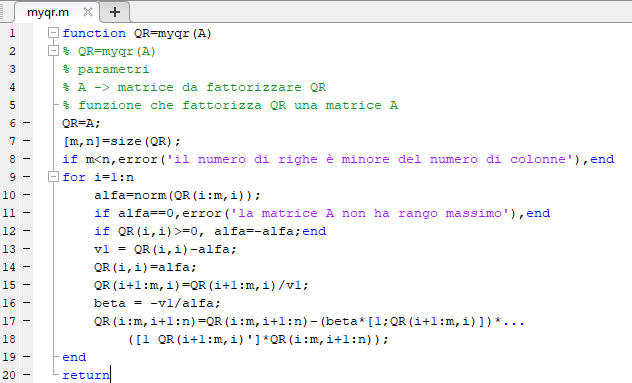
\includegraphics[width=1.3\linewidth]{img/myqr.png}\newpage